\documentclass[11pt,a4paper]{article}
\usepackage[T1]{fontenc}
\usepackage[utf8]{inputenc}
\usepackage{lmodern,microtype}
\usepackage[margin=25mm]{geometry}
\usepackage{amsmath,amssymb,amsthm,mathtools}
\usepackage{graphicx,booktabs,array,tabularx}
\usepackage[numbers,sort&compress]{natbib}
\usepackage[section]{placeins}
\usepackage{xcolor}
\usepackage[colorlinks=true,linkcolor=blue!45!black,citecolor=blue!45!black,urlcolor=blue!45!black]{hyperref}
\usepackage{url}
\setlength{\emergencystretch}{2em}
\newcommand{\Tr}{\operatorname{Tr}}
\newcommand{\id}{\mathbb{I}}
\newcommand{\dd}{\mathrm{d}}
\newcommand{\ket}[1]{\lvert #1\rangle}
\newcommand{\bra}[1]{\langle #1\rvert}
\newcommand{\norm}[1]{\lVert #1\rVert}
\newcommand{\E}{\mathcal{E}}
\newcommand{\R}{\mathcal{R}}
\newtheorem{proposition}{Proposition}
% Edit these fields before submission; no author identity is inferred.
\newcommand{\papertitle}{Spin phase-space quantum diffusion:\\multipole structure and mode recovery on the sphere}
\newcommand{\paperauthors}{Author names and affiliations to be supplied}
\newcommand{\paperdate}{Research manuscript draft --- 7 October 2026}

\hypersetup{pdftitle={Spin phase-space quantum diffusion: multipole structure and mode recovery on the sphere},pdfsubject={Finite-dimensional quantum generative model and controlled numerical study}}
% Generated by scripts/build_assets.py; do not edit.
\newcommand{\HybridRankReduction}{80.3}
\newcommand{\HybridTraceReduction}{51.1}
\newcommand{\AuditDecay}{$8.33\times10^{-16}$}
\newcommand{\AuditTrace}{$3.95\times10^{-14}$}
\newcommand{\AuditHerm}{$2.80\times10^{-16}$}
\newcommand{\AuditMinEigen}{$6.07\times10^{-5}$}
\newcommand{\AuditKraus}{$2.35\times10^{-14}$}
\newcommand{\AuditTwoDelta}{$2.08\times10^{-13}$}
\newcommand{\AuditMetricDelta}{$2.69\times10^{-14}$}

\title{\papertitle}
\author{\paperauthors}
\date{\paperdate}
\begin{document}
\maketitle
\begin{abstract}
We formulate a generative model for directional data using spin coherent states, isotropic open-system diffusion, and trainable quantum channels. Classical distributions on the sphere are encoded as mixed spin-$j$ states, whose irreducible multipoles evolve with the spherical heat spectrum $\exp[-D\ell(\ell+1)t]$ up to rank $2j$. We derive the encoding--diffusion correspondence and explicitly distinguish the input density from its finite-resolution Husimi readout. Exact density-matrix simulations then separate representational resolution, initialization, supervision, and optimization budget. In a 40-run paired study at $j=5/2$, an unchanged 162-parameter reverse architecture recovers both encoded target modes in five of five seeds with final-only fidelity training at 100 epochs, compared with one of five under path supervision. A hybrid fidelity--multipole objective selected on separate validation seeds reduces mean high-rank squared error by \HybridRankReduction\% and mean trace distance by \HybridTraceReduction\% on five new confirmation seeds; both objectives recover both modes in all five runs. A two-spin pilot demonstrates the product-phase-space construction but performs worse than correlation-aware classical baselines. These results establish a reproducible finite-dimensional prototype and expose training and representation limitations. They do not establish quantum advantage, hardware efficiency, or a benefit of diffusion supervision over direct state preparation.
\end{abstract}

\section{Introduction}
Diffusion models learn generative transformations by connecting structured data to a tractable noisy reference distribution \citep{ho2020}. For directional observations, the sphere supplies a natural geometry, and intrinsic diffusion methods already extend classical score-based generation to manifolds \citep{debortoli2022}. A quantum formulation can likewise exploit a physical phase space rather than treating directions as arbitrary strings of basis labels. A spin-$j$ system offers precisely such a representation: its coherent states are indexed by the sphere, while the finite operator algebra resolves a hierarchy of angular multipoles.

Quantum diffusion itself is established prior work. QuDDPM learns ensembles of quantum data using scrambling and measurement-based denoising \citep{zhang2024}; QGDM constructs non-unitary channel-based generation of mixed-state targets \citep{chen2026qgdm}. Quantum-noise-driven generative models include quantum and hybrid forward/backward formulations \citep{parigi2024}, and mixed-state QuDDPM uses quantum noise channels and measured reverse circuits \citep{kwun2024}. QD3PM addresses discrete classical joint distributions through quantum diffusion \citep{chen2026qd3pm}. These precedents rule out identifying the present construction as the first quantum, fully quantum, or classical-data quantum diffusion model.

Our focus is the combination of a spin phase-space representation with a multipole-resolved physical diffusion and an auditable generative reconstruction. The coherent-state formalism \citep{arecchi1972} and quantum dynamical semigroups \citep{lindblad1976} are standard, as are phase-space methods for dissipative spin systems \citep{merkel2021}. We therefore treat the heat-spectrum correspondence as a mathematical foundation used by the model, not as a newly discovered property of angular momentum. The contribution is the explicit construction, its controlled training diagnosis, and a record connecting claims to reproducible numerical evidence. We make no priority claim for their combination based on the targeted literature search alone.

Three questions organize the experiments. First, which classical structures survive coherent-state encoding and readout at a given $j$? Second, once a secondary mode is representable, does failure to generate it reflect the noisy starting state, the reverse architecture, the objective, or the training budget? Third, does the product-phase-space extension learn correlations competitively in a small two-spin example? The first two questions yield positive but narrowly scoped results. The third yields a negative pilot result that limits extrapolation to many-body generation.

Throughout, ``quantum'' describes the state and channel model. Training, density evolution, and readout sampling are performed on a classical computer. Each single-spin run fits one empirical mixed state and generates directions through its Husimi distribution. It does not learn a distribution over individually labelled quantum training states in the ensemble-learning sense of QuDDPM.

\section{Spin phase-space construction}
\subsection{Encoding and the observable distribution}
Let $\dd\Omega=\sin\theta\,\dd\theta\,\dd\phi$ denote surface area on the unit sphere and let $p$ be a normalized density with respect to this measure. Set $d=2j+1$, $\hbar=1$, and define
\begin{equation}
 \ket{\Omega}_j=e^{-i\phi J_z}e^{-i\theta J_y}\ket{j,j},\qquad
 \E_j[p]=\rho_p=\int_{S^2}p(\Omega)\ket{\Omega}\bra{\Omega}\,\dd\Omega.
 \label{eq:encoding}
\end{equation}
For $N$ observed directions, the empirical target is $\widehat\rho_0=N^{-1}\sum_a\ket{\Omega_a}\bra{\Omega_a}$. Coherent states resolve the identity,
$\frac{d}{4\pi}\int\ket{\Omega}\bra{\Omega}\,\dd\Omega=\id_d$,
so their positive operator-valued measure gives the normalized readout density
\begin{equation}
 q_\rho(\Omega)=\frac{d}{4\pi}\bra{\Omega}\rho\ket{\Omega},\qquad
 \int q_\rho(\Omega)\,\dd\Omega=1.
 \label{eq:readout}
\end{equation}
We use $q_\rho$ for the normalized Husimi density, avoiding an ambiguity between conventions for the unnormalized $Q$ symbol.

Encoding followed by readout smooths the input:
\begin{equation}
 q_{\rho_p}(\Omega)=\int K_j(\Omega\cdot\Omega')p(\Omega')\,\dd\Omega',\quad
 K_j(u)=\frac{2j+1}{4\pi}\left(\frac{1+u}{2}\right)^{2j}.
 \label{eq:kernel}
\end{equation}
Thus the observable target is generally not $p$. If $p=\sum_{\ell m}a_{\ell m}Y_{\ell m}$ in orthonormal spherical harmonics, the readout multiplies each coefficient by
\begin{equation}
 b_{j\ell}=\frac{(2j+1)[(2j)!]^2}{(2j-\ell)!(2j+\ell+1)!},\quad 0\leq\ell\leq2j,
 \qquad b_{j\ell}=0\quad(\ell>2j).
 \label{eq:transfer}
\end{equation}
In particular $b_{j0}=1$ and $b_{j1}=j/(j+1)$. Even retained modes are attenuated. The cutoff alone does not characterize usable resolution. The positive coefficients below the cutoff make the encoding injective on the truncated harmonic space, but high-rank inversion amplifies errors, and information above $2j$ is absent. Mixedness reflects averaging over nonorthogonal coherent states; its von Neumann entropy is not the differential entropy of $p$.

\subsection{Exact spherical heat evolution at finite resolution}
We choose the isotropic generator
\begin{equation}
 \mathcal L_j(\rho)=-D\sum_{\alpha=x,y,z}[J_\alpha,[J_\alpha,\rho]],\qquad D>0.
 \label{eq:lindblad}
\end{equation}
It has Lindblad operators $\sqrt{2D}J_\alpha$, so $\Phi_t=e^{t\mathcal L_j}$ is completely positive and trace preserving (CPTP) \citep{lindblad1976}. It is unital and covariant under rotations. This covariance concerns the forward process; the trained reverse maps need not be rotation covariant.

The operator space decomposes into irreducible tensor sectors $T_{\ell m}$ with $0\leq\ell\leq2j$. We choose $T_{00}=\id_d/\sqrt d$ and $\Tr(T_{\ell m}^\dagger T_{\ell' m'})=\delta_{\ell\ell'}\delta_{mm'}$. With $c_{\ell m}=\Tr(\rho T_{\ell m}^\dagger)$,
\begin{align}
 \sum_\alpha[J_\alpha,[J_\alpha,T_{\ell m}]]&=\ell(\ell+1)T_{\ell m},\nonumber\\
 c_{\ell m}(t)&=e^{-D\ell(\ell+1)t}c_{\ell m}(0),\label{eq:decay}\\
 P_\ell(t):=\sum_m|c_{\ell m}(t)|^2&=e^{-2D\ell(\ell+1)t}P_\ell(0).\nonumber
\end{align}
Higher ranks decay faster. Only the scalar sector survives asymptotically, giving $\rho_t\to\id_d/d$.

\begin{proposition}[Encoding--heat intertwining]
Let $H_t=e^{tD\Delta_{S^2}}$ be the spherical heat semigroup. Then
\begin{equation}
 \Phi_t\E_j[p]=\E_j[H_t p],\qquad
 q_{\Phi_t(\rho)}=H_tq_\rho.
 \label{eq:intertwine}
\end{equation}
\end{proposition}
\begin{proof}
The map $\E_j$ is rotation equivariant because coherent projectors transform by conjugation. The spin-$j$ operator space contains one copy of each rank $\ell=0,\ldots,2j$ and no higher ranks. Equivariance maps each retained spherical-harmonic sector to its tensor sector up to a scalar, and annihilates the rest. On either retained sector, the respective generator has eigenvalue $-D\ell(\ell+1)$; exponentiating proves the first identity. The readout is also equivariant, so the same sector argument proves the second. Equivalently, the rotation-invariant kernel in Eq.~\eqref{eq:kernel} commutes with heat evolution.
\end{proof}
The correspondence is exact on the encoded representation. It is not an equivalence between unrestricted classical densities and finite-dimensional quantum states. Nor does the ordering of forward decay prove that a learned reverse stack restores ranks in a prescribed order.

\subsection{Physical reverse maps and sampling}
Each reverse step introduces a fresh pure ancilla, applies a trainable joint unitary, and discards the ancilla:
\begin{equation}
 \R_s(\rho)=\Tr_a\!\left[U_s(\rho\otimes\ket0\bra0)U_s^\dagger\right]
 =\sum_kK_{s,k}\rho K_{s,k}^\dagger,\quad K_{s,k}=\bra kU_s\ket0.
 \label{eq:reverse}
\end{equation}
This is CPTP by construction; state renormalization or positive-semidefinite projection is not part of the map. The generative state is $\rho_{\rm gen}=\R_S\circ\cdots\circ\R_1(\id_d/d)$. Pure fresh ancillas allow this stack to reduce the system entropy despite starting from the maximally mixed prior.

The reverse is target dependent, not a universal inverse of heat diffusion. Such an inverse would amplify distinguishability lost by a channel and need not be positive. In the present simulation, one trained stack prepares one target mixed state. Sampling $q_{\rho_{\rm gen}}$ then produces classical directions.

Measuring the ancilla instead gives a quantum instrument. Outcome $k$ has probability $p_k=\Tr(K_k\rho K_k^\dagger)$ and conditional state $\rho_k=K_k\rho K_k^\dagger/p_k$ for $p_k>0$. The equality $\sum_kp_k\rho_k=\R(\rho)$ holds exactly. Different conditional trajectories form one decomposition of the output density, but recovering that density does not identify a unique source ensemble. Both instrument sampling and the coherent-state POVM are operational definitions; the experiments use matrix simulation and a finite readout grid rather than a hardware measurement implementation.

\subsection{Correlated product phase spaces}
For directions on $(S^2)^n$, define
\begin{equation}
 \rho_p=\int p(\Omega_1,\ldots,\Omega_n)
 \bigotimes_{i=1}^n\ket{\Omega_i}\bra{\Omega_i}\,\prod_i\dd\Omega_i.
 \label{eq:joint}
\end{equation}
The local forward generator is the sum of the single-spin generators. Product tensors have eigenvalues $-\sum_iD_i\ell_i(\ell_i+1)$ and therefore separate local angular resolution from joint correlations. However, every state encoded by Eq.~\eqref{eq:joint} is separable across the spin subsystems. Classical dependence can yield nonzero connected correlations and quantum mutual information without entanglement. A reverse circuit may access entangled states, but neither their necessity nor their usefulness is demonstrated here. Dense simulation stores $\prod_i(2j_i+1)^2$ matrix entries, which grows exponentially with the number of spins.

\section{Numerical methods and experimental design}
\subsection{Data, representation, and architecture}
The single-spin source draws either of two unit directions with equal probability,
\begin{equation}
 \mu_1=(0.8,0,0.6),\qquad
 \mu_2=\frac{(-0.4,0.7,0.6)}{\norm{(-0.4,0.7,0.6)}}.
\end{equation}
A sample is $x=(\mu_z+\sigma\epsilon)/\norm{\mu_z+\sigma\epsilon}$, with $\epsilon\sim\mathcal N(0,\id_3)$ and $\sigma=0.22$. This is a normalized Gaussian mixture, not an exact von Mises--Fisher sampler. Each seed supplies $N=2000$ directions and its own empirical density. Single-spin evaluation compares against that same empirical encoded target. New confirmation seeds are independent data realizations and parameter initializations, not held-out observations from the training dataset of a fixed model.

A representation sweep uses the seed-7 dataset and $j\in\{1/2,1,3/2,2,5/2,3,4,5\}$. Subsequent controlled experiments use $j=5/2$, dimension six, with six forward time steps, $D=1$ and $\Delta t=0.35$. Matrix exponentiation of the Liouvillian gives the forward trajectory $\rho_0,\ldots,\rho_6$ at times $t_s=s\Delta t$.

Each reverse unitary has three layers and nine ordered Hermitian generators:
\begin{equation}
 \{J_x\otimes\id,J_y\otimes\id,J_z\otimes\id,J_z^2\otimes\id,
 J_x\otimes X,J_y\otimes Y,J_z\otimes Z,\id\otimes X,\id\otimes Y\}.
 \label{eq:generators}
\end{equation}
Every generator is divided by its Hilbert--Schmidt norm. Exponentials are multiplied in the order implemented by the archived source; parameters are independent across steps. There are $6\times3\times9=162$ real parameters. The ansatz acts within the spin-$j$ representation. Preservation of this representation does not imply rotational covariance of the learned channel.

Angles are initialized independently as $0.03\,\mathcal N(0,1)$ and optimized with Adam at learning rate $0.04$, default $\beta_1=0.9$, $\beta_2=0.999$, and $\epsilon=10^{-8}$ \citep{kingma2015}. Training uses double-precision real parameters and complex-double matrices. The same seed fixes the target and initialization across each paired diagnostic condition.

\subsection{Supervision and objectives}
Let $\widetilde\rho_s=\R_s\circ\cdots\circ\R_1(\pi)$ be the state after $s$ reverse steps, for $\pi=\id_d/d$ or, diagnostically, $\pi=\rho_6$. For a state loss $L$, the two objectives are
\begin{equation}
 L_{\rm path}=\sum_{s=1}^{6}L(\widetilde\rho_s,\rho_{6-s}),\qquad
 L_{\rm final}=L(\widetilde\rho_6,\rho_0).
 \label{eq:supervision}
\end{equation}
Path training backpropagates through the composed stack: it is not teacher-forced training of isolated one-step inverse channels. The path sum is not divided by six. Consequently the comparison changes both the intermediate constraints and the overall loss scale; it does not isolate a gradient-conflict mechanism.

The diagnostic loss is squared-Uhlmann infidelity,
\begin{equation}
 L_F(\rho,\sigma)=1-F(\rho,\sigma),\qquad
 F(\rho,\sigma)=\left[\Tr\sqrt{\sqrt\rho\,\sigma\sqrt\rho}\right]^2.
\end{equation}
The follow-up objective is $L_\lambda=(1-\lambda)L_F+\lambda L_M$, where
\begin{equation}
 L_M=\sum_{\ell=0}^{2j}w_\ell\sum_{m=-\ell}^{\ell}
 |c_{\ell m}(\rho)-c_{\ell m}(\sigma)|^2,\qquad
 w_\ell=\frac{d^2(\ell+1)^2}{\sum_{r=0}^{2j}(2r+1)(r+1)^2}.
 \label{eq:hybrid}
\end{equation}
Weights have mean one over all $d^2$ components. Uniform component weights reproduce squared Frobenius distance by Parseval's identity. Although $L_M$ emphasizes high ranks, it includes all accessible ranks. The separate selection metric $E_{45}=\sum_{\ell=4}^{5}\sum_m|\Delta c_{\ell m}|^2$ measures only the top two ranks at $j=5/2$.

\subsection{Controlled study and confirmation protocol}
The diagnostic crosses two starting states, two supervision schemes, and two budgets (100 or 500 epochs), for seeds $3,5,7,11,13$: 40 runs in total. Starting at $\rho_6$ uses target information and is an initialization diagnostic, not sampling from a target-independent prior. Both starts are evaluated separately; the mixed-prior output of every trained model is also archived.

The hybrid study uses final supervision, the mixed prior, and 500 epochs. Its saved protocol fixes candidate weights $\lambda\in\{0,0.25,0.5,0.75\}$ and validation seeds $17,19,23,29,31$. A candidate is eligible if its mean infidelity, trace distance and Husimi-grid Jensen--Shannon (JS) divergence worsen relative to $\lambda=0$ by no more than $0.005$, $0.01$ and $0.001$, respectively. Among eligible candidates, selection maximizes the number of runs recovering both modes, then minimizes mean $E_{45}$, then favors the smaller $\lambda$. Selection is saved before comparing the selected value and zero on confirmation seeds $41,43,47,53,59$. There are 20 validation and 10 confirmation runs. This is a repository-recorded predeclared protocol, not an externally registered study.

\subsection{Metrics and mode detection}
We report squared Frobenius error $\norm{\rho-\sigma}_F^2$, trace distance $\frac12\norm{\rho-\sigma}_1$, infidelity and JS divergence in nats. For JS, the $80\times160$ angular grid is converted into probability masses using $q(\theta,\phi)\sin\theta$ and normalized; $10^{-14}$ stabilization is then added before a second normalization. A high correlation between unweighted $q$ grids is a global descriptive statistic, not a mode-recovery test.

Significant modes are maxima in a $5\times5$ grid neighborhood, with periodic azimuth and nearest-value polar boundaries. Candidates must reach half the global maximum; descending-height suppression imposes at least $0.35$ radians separation. A minimum-total-angle one-to-one assignment matches generated and target modes, and only assigned angles of at most $0.35$ radians count as recovered. Missing peaks are not replaced by the value of $q$ near their expected location. These choices are fixed across the experiments. The criterion is a grid diagnostic rather than a topological or resolution-independent definition of modality.

Tables use means and sample standard deviations across seeds unless otherwise indicated. Paired effects and descriptive Student-$t$ intervals are provided in the evidence bundle; no multiplicity-adjusted hypothesis tests or population success-rate claims are made. Five seeds characterize this small experiment, not a broad class of directional distributions.

\subsection{Two-spin pilot and classical comparators}
The pilot uses two $j=1$ spins, 1200 training pairs, and 1200 independent test pairs. The first direction follows the mixture above with $\sigma=0.18$; the second is a normalized Gaussian perturbation of the first rotated by $0.55$ radians around $z$. Training seed 17 and test seed 1017 define one split. The local forward process has three steps, $D=1$, $\Delta t=0.5$. Both quantum models use one layer per reverse step, a shared ancilla, fidelity path supervision, 80 epochs and learning rate $0.04$. Adding $J_{z1}J_{z2}$ and $J_{x1}J_{x2}+J_{y1}J_{y2}$ generators increases parameters from 33 to 39. The shared ancilla can already mediate correlations in the model without direct interactions.

The comparators are the product of training marginals; a spherical kernel estimator with bandwidth $0.10$; a two-component separable product mixture; and a 39-parameter neural generator trained for 300 epochs to match first and second moments. The kernel estimator bootstraps paired observations and perturbs each direction with a tangent-plane Gaussian mapped onto the sphere. The code labels it ``Riemannian heat-kernel KDE,'' but it is a finite-increment approximation, not an exact spectral heat-kernel sampler or a learned reverse diffusion. Parameter matching of the neural and direct-interaction quantum models does not match training objectives or compute. Metrics use the encoded independent test state, quantum mutual information $I(A:B)=S(\rho_A)+S(\rho_B)-S(\rho_{AB})$, and the Frobenius error of the connected $3\times3$ spin-correlation tensor.

The current repository additionally implements an ambient-space classical DDPM with normalization onto the sphere. It was added after the archived studies and has no results in this paper's frozen evidence. We do not substitute that implementation for a completed comparison. A competitive single-spin benchmark against learned classical diffusion remains outstanding.

\section{Results}
\subsection{Resolution and exact forward dynamics}
Under the declared grid criterion, the seed-7 encoded target has one significant maximum for $j\leq2$ and two starting at $j=5/2$ (Fig.~\ref{fig:physics}). This motivates dimension six for the training diagnosis; it is not a universal threshold for resolving two spherical modes. Encoding and readout smooth the particular data through Eq.~\eqref{eq:kernel}.

Across all 70 diagnostic and hybrid runs, a fresh coefficient audit gives a maximum absolute forward-decay error of \AuditDecay. Saved forward and reverse states have maximum trace residual \AuditTrace, maximum Hermiticity residual \AuditHerm, and minimum eigenvalue \AuditMinEigen. Replaying the stored parameters reproduces the saved generated states to the precision reported in the audit; the maximum Kraus-completeness residual is \AuditKraus. These are numerical consistency checks, not a substitute for the analytic CPTP argument.

\begin{figure}[tbp]
 \centering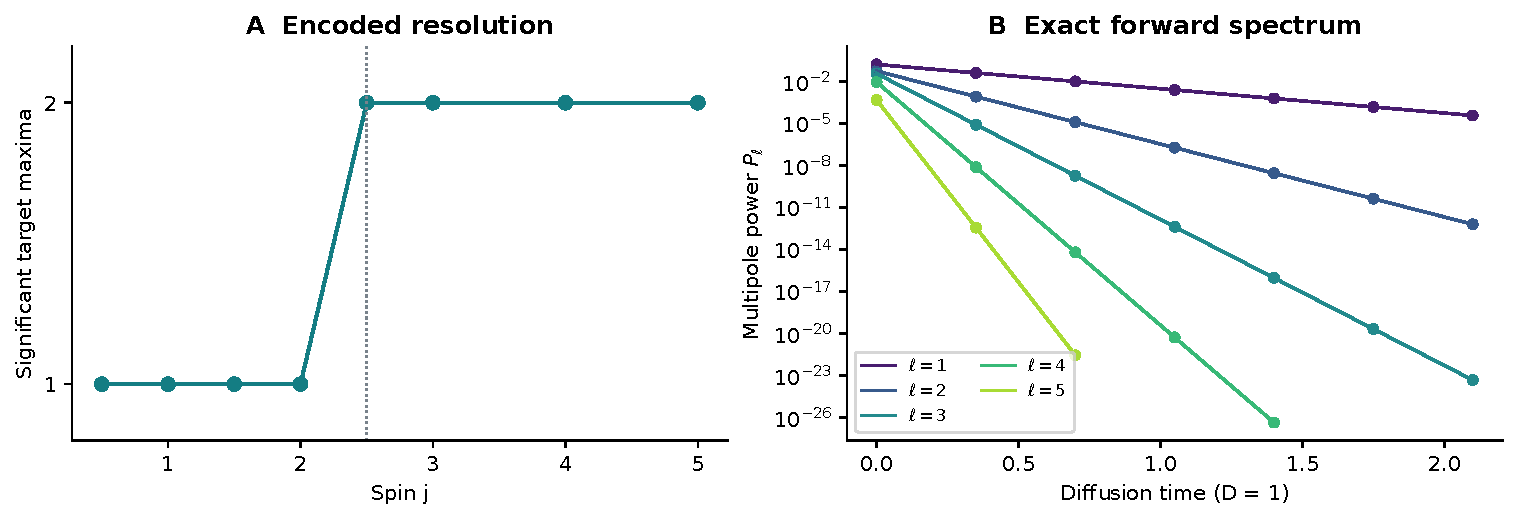
\includegraphics[width=\linewidth]{figures/physics.pdf}
 \caption{Finite resolution and forward diffusion. Left: significant maxima in the encoded target for the fixed seed-7 dataset. Right: measured multipole powers (markers) and the exact decay law (lines), using the seed-7 $j=5/2$ forward trajectory. Values below $10^{-28}$ are omitted from the logarithmic plot because floating-point residuals dominate. All retained ranks are present in the saved data.}
 \label{fig:physics}
\end{figure}

\subsection{Final supervision resolves the missing-mode failure}
Table~\ref{tab:diagnostic} reports every condition in the paired 40-run diagnostic. At 100 epochs, fidelity path supervision recovers both modes in one of five seeds for either start. Final-only supervision recovers both in all five. For the generative mixed prior, mean infidelity falls from approximately $4.21\times10^{-2}$ to $7.17\times10^{-4}$ and mean trace distance from $0.1328$ to $0.0161$. Switching to the exact terminal forward state does not remove the path-training failure.

\begin{table}[tbp]
 \centering\small
 \caption{Controlled diagnostic at $j=5/2$. Each row summarizes the same five seeds. Entries are mean $\pm$ sample standard deviation; mode counts are successes out of five. $\rho_6$ is the target-dependent terminal forward state.}
 \label{tab:diagnostic}
 \begin{tabular}{lllcrr}
\toprule
Start & Loss & Epochs & Modes & Infidelity & Trace distance \\
\midrule
$\id/d$ & path & 100 & 1/5 & $0.0421\pm0.0132$ & $0.1328\pm0.0257$ \\
$\id/d$ & final & 100 & 5/5 & $(7.17\pm3.73)\,10^{-4}$ & $0.0161\pm0.0059$ \\
$\rho_6$ & path & 100 & 1/5 & $0.0422\pm0.0121$ & $0.1334\pm0.0234$ \\
$\rho_6$ & final & 100 & 5/5 & $(8.35\pm4.46)\,10^{-4}$ & $0.0176\pm0.0067$ \\
$\id/d$ & path & 500 & 5/5 & $0.0122\pm0.0011$ & $0.0690\pm0.0062$ \\
$\id/d$ & final & 500 & 5/5 & $(2.98\pm2.26)\,10^{-5}$ & $(3.05\pm0.62)\,10^{-3}$ \\
$\rho_6$ & path & 500 & 5/5 & $0.0112\pm0.0007$ & $0.0650\pm0.0059$ \\
$\rho_6$ & final & 500 & 5/5 & $(2.70\pm1.16)\,10^{-5}$ & $(3.12\pm1.13)\,10^{-3}$ \\
\bottomrule
\end{tabular}

\end{table}

At 500 epochs, all four conditions recover both modes, but the final-only objective retains substantially lower state error. Rank-resolved errors likewise reveal structure missed by global visual similarity (Fig.~\ref{fig:diagnostic}). In the original 100-epoch mixed-prior path runs, correlations of the generated and target Husimi grids exceed $0.995$ even in failures. High correlation alone is therefore insufficient evidence of multimodal recovery.

\begin{figure}[tbp]
 \centering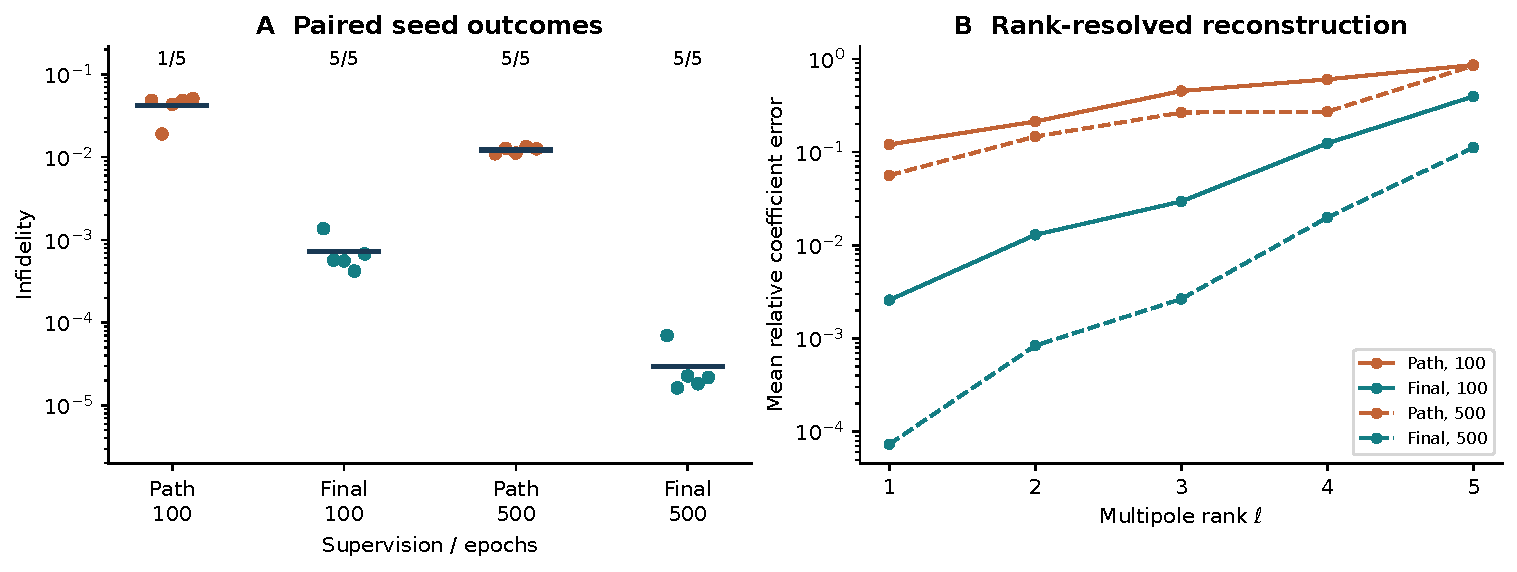
\includegraphics[width=\linewidth]{figures/diagnostic.pdf}
 \caption{Training diagnosis for the generative mixed prior. Left: individual-seed infidelity and group means for the two objectives and epoch budgets; annotations give both-mode recovery. Right: mean relative coefficient error by rank, retaining phase and orientation information. Each curve aggregates the same five seeds. These are descriptive paired experiments; the figure does not isolate a unique optimization mechanism.}
 \label{fig:diagnostic}
\end{figure}

These results show that the fixed architecture can represent a successful generated state for this problem. They support the supervision choice and optimization budget as practical limitations of the original run. They do not establish a general superiority of final-only objectives: scale normalization, alternative learning rates, and intermediate-state gradient interactions were not separately controlled. Moreover, final-only training uses no intermediate forward targets; its success is also consistent with a deep dissipative state-preparation model.

\subsection{Validation-selected multipole weighting improves high-rank accuracy}
The saved selection rule chooses $\lambda=0.75$. Both the selected hybrid and pure fidelity recover both modes for all five confirmation seeds. Table~\ref{tab:hybrid} shows all validation candidates and both confirmation conditions. On confirmation, mean $E_{45}$ decreases from $1.4272\times10^{-5}$ to $2.8103\times10^{-6}$, a \HybridRankReduction\% reduction. Mean trace distance falls by \HybridTraceReduction\%, from $0.003612$ to $0.001767$. The mean JS divergence increases by approximately $7.48\times10^{-8}$, within the predeclared absolute guardrail. Thus the improvement concerns reconstruction accuracy rather than the already saturated binary mode count.

\begin{table}[tbp]
 \centering\small
 \caption{Hybrid selection and confirmation. Each row contains five seeds; all rows recover both modes in five of five runs. Entries are means, with per-seed values and uncertainty in the archive. $E_{45}$ is the squared error of rank-4 and rank-5 coefficients. Confirmation seeds were not used to choose $\lambda$.}
 \label{tab:hybrid}
 \begin{tabular}{llrrrr}
\toprule
Split & $\lambda$ & Infidelity & Trace distance & JS (nats) & $E_{45}$ \\
\midrule
Validation & 0 & $3.28\times10^{-5}$ & $3.48\times10^{-3}$ & $9.35\times10^{-7}$ & $1.54\times10^{-5}$ \\
Validation & 0.25 & $3.57\times10^{-5}$ & $3.18\times10^{-3}$ & $1.08\times10^{-6}$ & $1.24\times10^{-5}$ \\
Validation & 0.5 & $2.83\times10^{-5}$ & $2.20\times10^{-3}$ & $7.78\times10^{-7}$ & $4.92\times10^{-6}$ \\
Validation & 0.75 & $3.33\times10^{-5}$ & $1.75\times10^{-3}$ & $8.37\times10^{-7}$ & $2.59\times10^{-6}$ \\
Confirmation & 0 & $3.52\times10^{-5}$ & $3.61\times10^{-3}$ & $1.02\times10^{-6}$ & $1.43\times10^{-5}$ \\
Confirmation & 0.75 & $2.96\times10^{-5}$ & $1.77\times10^{-3}$ & $1.10\times10^{-6}$ & $2.81\times10^{-6}$ \\
\bottomrule
\end{tabular}

\end{table}
\begin{figure}[tbp]
 \centering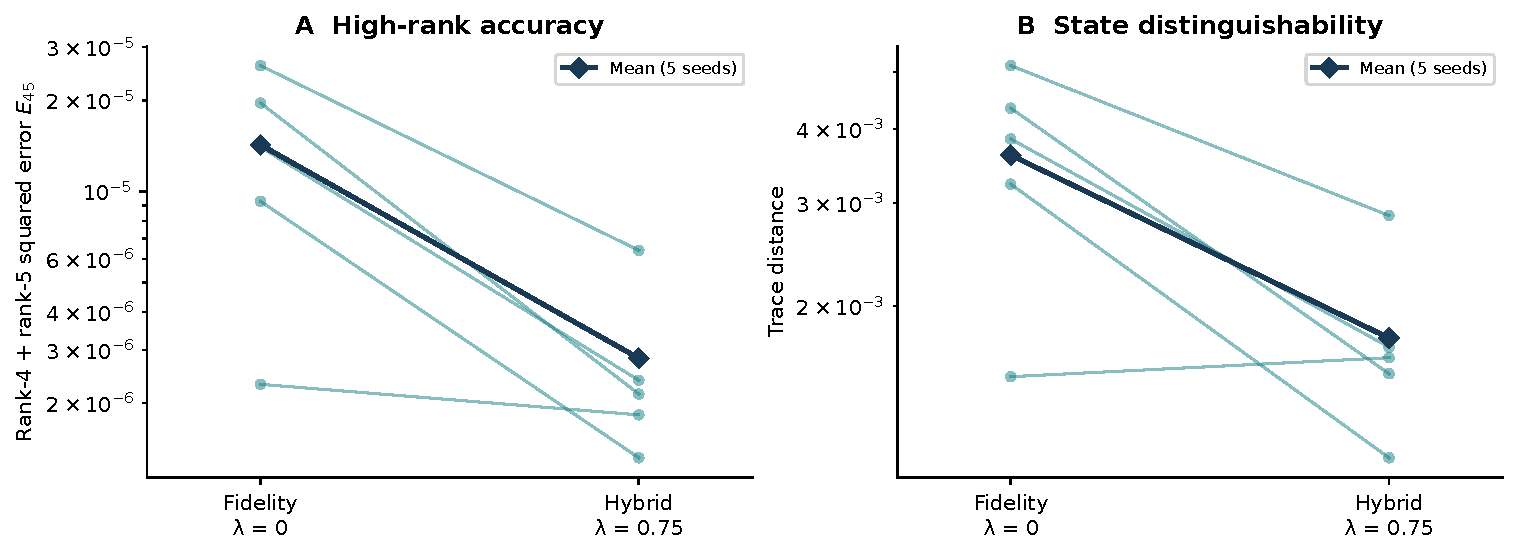
\includegraphics[width=\linewidth]{figures/hybrid.pdf}
 \caption{Paired confirmation outcomes at 500 epochs. Lines connect the same seed under pure fidelity and the selected hybrid; dark markers give the group means. The reduction in the means does not imply improvement on every individual seed. Axes are logarithmic to show relative differences.}
 \label{fig:hybrid}
\end{figure}

\subsection{Instrument consistency and the correlated-model limitation}
The historical instrument study applies ancilla measurements to the five original 100-epoch $j=5/2$ fidelity models, using 256 trajectories per model. The mean squared Frobenius distance between the trajectory ensemble and deterministic channel output is $0.000701\pm0.000279$, and the mean trace distance is $0.02466\pm0.00540$. These sample fluctuations are compatible with the exact branch-average identity. They do not constitute a demonstrated sampling-speed benefit. The archive contains the aggregate instrument tables; individual conditional trajectories were not retained, so these ensemble values are preserved historical results rather than a fresh trajectory-level audit.

The independent test state in the two-spin pilot has quantum mutual information $0.34454$ nats. The factorized baseline loses this dependence, but both learned quantum models are less accurate even than that baseline in trace distance (Table~\ref{tab:two}). Direct interactions improve the quantum results slightly; they do not close the much larger gap to the spherical kernel, separable mixture, or neural generator. The six saved model states pass a fresh independent metric comparison with maximum discrepancy \AuditTwoDelta.

\begin{table}[tbp]
 \centering\small
 \caption{Two-spin pilot, one independent train/test split. Parameter counts distinguish trainable (t) from effective (e) counts. Errors compare to the same encoded test state; MI is quantum mutual information in nats. Different training budgets and objectives preclude a resource-matched advantage claim.}
 \label{tab:two}
 \begin{tabular}{lrrrr}
\toprule
Model & Parameters & Trace dist. & MI error & Corr. error \\
\midrule
Factorized marginals & 16 e & 0.3272 & 0.3445 & 0.4525 \\
Spherical kernel & 0 t & 0.0342 & 0.0139 & 0.0157 \\
Separable mixture & 33 e & 0.0405 & 0.0468 & 0.0391 \\
Quantum, no direct & 33 t & 0.5328 & 0.3253 & 0.4849 \\
Quantum, direct & 39 t & 0.5286 & 0.3195 & 0.4623 \\
Neural generator & 39 t & 0.0526 & 0.0431 & 0.0324 \\
\bottomrule
\end{tabular}

\end{table}
The two-spin experiment therefore establishes an implemented correlated extension and a baseline comparison, not successful competitive many-body generation. It also cannot attribute a role to entanglement: the target encoding is separable and no entanglement ablation was performed.

\section{Discussion and limitations}
The representation supplies a direct relation between spherical geometry, angular resolution, and physical noise. Multipole coefficients expose reconstruction errors that total-state losses and global Husimi correlation can conceal. The controlled experiment also changes the interpretation of an initial missing-mode result: failure at a short training budget does not establish an expressivity limit of the channel family.

The scope remains deliberately small. The data consist of one synthetic mixture family. Single-spin errors are empirical reconstruction errors, and the confirmation split measures repeatability across newly sampled datasets rather than out-of-sample generalization of a frozen model. Finite-$j$ encoding discards high harmonics and attenuates lower ones; even exact density reconstruction generates the smoothed readout, not the original density. A grid-dependent mode criterion adds further resolution dependence.

Several comparisons are necessary before attributing a generative benefit to diffusion. Final-only training uses a composition of physical channels but no intermediate forward targets. A matched single-channel or direct state-preparation baseline, a normalized path loss, and a learned classical spherical diffusion baseline would distinguish the role of the forward construction from that of parameterized state preparation. The present data cannot demonstrate that the six-stage structure is necessary. Likewise, the forward spectrum orders decay but does not establish coarse-to-fine ordering of the learned reverse dynamics.

The correlated pilot is a clear current limitation. Additional reverse capacity, improved supervision, or different ancilla designs might help, but no such improvement is claimed without experiments. Multiple independent train/test splits and jointly reported state, correlation, parameter, compute and sampling costs are needed. Classical correlations in the source already admit a separable encoded representation, so an exponential Hilbert-space dimension alone is not evidence of a quantum computational advantage.

Hardware execution is also untested. The spin-$j$ space can be represented as the symmetric sector of $2j$ qubits, but a physical device requires specific preparation, control, reset, and readout implementations. The simulated coherent-state POVM and dense matrix trajectory do not supply gate-depth estimates or a scalable sampling procedure. The work supports an operationally quantum model implemented in simulation, not a demonstrated hardware-native generator.

\section{Conclusion}
Spin coherent-state encoding and isotropic Lindblad diffusion give a finite-dimensional generative construction with an exact spherical heat spectrum. The numerical evidence separates representation limits from training failures: final-only supervision restores the representable secondary mode without enlarging the reverse architecture, and validation-selected multipole weighting improves high-rank reconstruction on new seeds. The poor two-spin pilot and the absence of direct-preparation and learned classical diffusion comparisons define the immediate limits of the result. The accompanying evidence archive makes these positive and negative conclusions inspectable and provides a stable basis for extending the study.

\section*{Data and code availability}
The accompanying project includes frozen density matrices, parameters, configurations, study protocols, source snapshots, checksum manifests, and scripts that audit the principal results and regenerate every paper table and figure. A claim-to-evidence ledger identifies the support and limitations of each result. The 70-run diagnostic/hybrid source snapshot is contemporaneous; earlier studies have less complete source provenance, as recorded in the archive. No public repository URL or archival DOI has yet been designated. Author details, funding, contributions, competing-interest declarations, and a permanent public archive must be completed by the authors before submission.

\bibliographystyle{unsrtnat}
\bibliography{references}
\clearpage
\appendix
\section{Readout transfer function and tensor conventions}
The overlap of two spin coherent states is
$|\langle\Omega|\Omega'\rangle|^2=[(1+\Omega\cdot\Omega')/2]^{2j}$.
Rotational convolution and the Funk--Hecke formula give
\begin{equation}
 b_{j\ell}=\frac{2j+1}{2}\int_{-1}^{1}
 \left(\frac{1+u}{2}\right)^{2j}P_\ell(u)\,\dd u.
\end{equation}
Using Rodrigues' formula for $P_\ell$ and integrating by parts $\ell$ times yields Eq.~\eqref{eq:transfer}. If $\ell>2j$, the differentiated polynomial vanishes. This also explains why a resolution claim based only on the largest accessible rank would be incomplete.

The numerical tensors start at $T_{\ell\ell}\propto(-1)^\ell J_+^\ell$, normalized in Hilbert--Schmidt norm, and descend through
\begin{equation}
 T_{\ell,m-1}=\frac{[J_-,T_{\ell m}]}{\sqrt{(\ell+m)(\ell-m+1)}}.
\end{equation}
They obey $T_{\ell m}^\dagger=(-1)^mT_{\ell,-m}$ and reconstruct a state as $\rho=\sum_{\ell m}c_{\ell m}T_{\ell m}$. In an orthonormal spherical-harmonic convention with compatible phases, the encoding maps $Y_{\ell m}$ to a tensor with scalar magnitude $\sqrt{4\pi b_{j\ell}/d}$. The precise phase convention is immaterial to the spectrum but must be consistent when comparing individual coefficients.

\section{Physicality and numerical evaluation}
Every simulated state is checked for trace one, Hermiticity and positivity at tolerance $10^{-10}$. For each reverse step, Kraus completeness is checked, and historical run metadata also retain Choi-matrix minimum eigenvalues. Forward and deterministic reverse helpers do not renormalize or project states. Small negative eigenvalues may be clipped only when evaluating square roots in fidelity or grid probabilities within roundoff tolerances; this metric stabilization is not a repaired state trajectory.

An initial longer diagnostic attempt exceeded the existing unitarity tolerance using generic matrix exponentials. The completed study instead evaluates each fixed Hermitian generator through its cached eigendecomposition,
\begin{equation}
 G=V\operatorname{diag}(g_r)V^\dagger,\qquad
 e^{-i\vartheta G}=V\operatorname{diag}(e^{-i\vartheta g_r})V^\dagger.
\end{equation}
This preserves the channel ansatz and analytic angle derivatives. The interrupted attempt is excluded from the reported results. The paper archive uses only the consistent completed rerun; it does not pool the interrupted run with the 40 diagnostic runs. Original repository notes retain the numerical precheck history.

The manuscript audit hashes all frozen evidence files, re-evaluates primary state metrics with NumPy, rechecks mode assignments and coefficient errors, replays the archived reverse channels, and verifies forward decay and trajectory physicality for 70 runs. Tensor generation, peak finding and channel replay reuse historical implementation code, so these portions are consistency checks. State-distance calculations and the two-spin metric audit are independent of training-loss implementations. The fresh maximum state-metric discrepancy is \AuditMetricDelta.

\section{Statistical and provenance details}
The principal experimental unit is a seed, which changes both the finite data realization and the initial parameters. Conditions within a seed are paired. Sample standard deviations use denominator $n-1$. Descriptive paired intervals use $\bar\delta\pm t_{0.975,4}s_\delta/\sqrt5$. With only five seeds, these intervals should not be read as a comprehensive characterization of tails or robustness. The selection rule's guardrails are operational tolerances, not significance thresholds.

The historical $j=2$ objective sweep and $j=5/2$ fidelity study are retained in the evidence directory as background. Their 100-epoch defaults motivated the later controlled study; their results are not pooled with the 500-epoch confirmation results. Instrument aggregates likewise concern the original 100-epoch models. The two-spin pilot retains its separate source-provenance limitations and distinct training budget. Runtime measurements taken during concurrent execution are not isolated performance benchmarks.

The manuscript distinguishes three reproducibility levels. Saved-state auditing and regeneration of figures/tables use the frozen evidence without training. Replaying channels additionally requires the archived scientific implementation and PyTorch. Fresh training should use the historical source snapshot for exact protocol replication, or a new output directory with the current source for an explicitly updated experiment. The current source adds a classical DDPM; mixing its new outputs into old study folders would break provenance.

\end{document}
